\documentclass[11pt,letterpaper]{article}
\usepackage[lmargin=1in,rmargin=1in,bmargin=1in,tmargin=1in]{geometry}
\usepackage{../style}

\setlength{\parindent}{0ex}

% -------------------
% Content
% -------------------
\begin{document}

\pagenumbering{gobble}

% Recitation: Linear Functions Review Solutions
\phantom{} \hfill {\bfseries \Large Recitation: Linear Functions Review Solutions} \hfill \phantom{} \par\vspace{0.5cm}

% Problem 1
{\scriptsize
\noindent {\bfseries Problem 1.} A small tanker truck is depositing its gas at a storage facility. The tanker is carrying 11,600~gallons of gas and is emptying its tank at a rate of 528.3~gal/min. Let $G(t)$ denote the volume of gas, in thousands, left in the tanker $t$ minutes from now. 
	\begin{enumerate}[(a)]
	\item Explain why $G(t)$ is linear. 
	\item Find $G(t)$ and sketch it in the plot below. 
	\item Interpret the slope of $G(t)$.
	\item Interpret the $y$-intercept for $G(t)$.
	\item Find and interpret (if possible) the $x$-intercept for $G(t)$. 
	\end{enumerate}
}

{\small\itshape
\sol 
\begin{enumerate}[(a)]
\item The rate of change of $G(t)$, i.e. the rate at which gas is flowing out of the tanker, is constant. Therefore, $G(t)$ must be linear. \pspace

\item By (a), we know that $G(t)$ is linear. Therefore, $G(t)= mt + b$ for some $m, b$. We know $m$ is the rate of change of $G(t)$. We are told that gas is leaving the tanker at a rate of 528.3~gal/min, i.e. 0.5283~thousands of gallons per minute. But we must then have $m= -0.5283$ because the amount of gas in the tanker is \textit{decreasing} at a rate of 0.5283~thousands of gallons per minute. But then $G(t)= -0.5283t + b$. At the start, i.e. at $t= 0$, we know the tanker has 11,600~gallons of gas (11.6~thousands of gallons of gas), i.e. $G(0)= 11.6$. But then $11.6= G(0)= -0.5283(0) + b= b$. Therefore, $G(t)= -0.5283t + 11.6$. We sketch $G(t)$ on the plot below. \pspace

\item We know that $m= \frac{\Delta G}{\Delta t}$, i.e. the amount of change in the gallons of gas over time. Because $m= -0.5283 < 0$, we know that the amount of gas is decreasing. As $m= -0.5283$, the slope represents the fact that every minute, 0.5283~thousands of gallons of gas is emptied from the tanker, i.e. 528.3~gallons of gas are emptied from the tanker every minute. \pspace

\item The $y$-intercept is when $t= 0$~minutes. We have $G(0)= -0.5283(0) + 11.6= 11.6$. Therefore, the $y$-intercept represents the fact that at 0~minutes, the tanker is carrying 11.6~thousands of gallons of gas, i.e. there are initially 11,600~gallons of gas in the tanker. \pspace

\item The $x$-intercept occurs when $G(t)= 0$. But then we have\dots
	\[
	\begin{gathered}
	G(t)= 0 \\
	-0.5283t + 11.6= 0 \\
	-0.5283t= -11.6 \\
	t\approx 21.96 \text{ minutes}
	\end{gathered}
	\]
Therefore, $G(t)= 0$ when $t \approx 21.96$, i.e. the tanker is empty after 21.96~minutes. 
\end{enumerate}
}



	\hfill
	\fbox{
	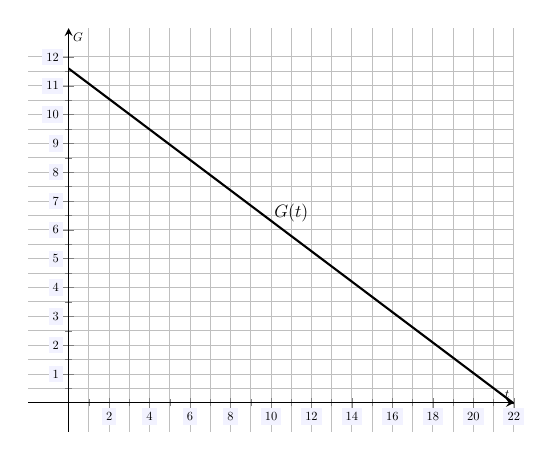
\begin{tikzpicture}[scale=0.9,every node/.style={scale=0.5}]
	\begin{axis}[
	grid=both,
	axis lines=middle,
	ticklabel style={fill=blue!5!white},
	xmin= -2, xmax=22,
	ymin= -1, ymax=13,
	xtick={0,2,...,22},
	ytick={0,1,2,...,12},
	minor x tick num = 1,
	minor y tick num = 1,
	xlabel=\(t\),ylabel=\(G\),
	]
	\node at (11,6.6) {\Large$G(t)$};
	\addplot[domain=0:22,samples=2,line width=0.03cm] (x, -0.5283*x+11.6);
	\end{axis}
	\end{tikzpicture}
	}
	


\newpage



% Problem 2
\noindent {\bfseries Problem 2.} Find the equation of the line with $x$-intercept 5 and $y$-intercept $-6$. \par\vspace{0.3cm}

\noindent{\itshape We want the equation of the line, which must have the form $y= mx + b$. We need a point and a slope. Because the $x$-intercept is 5, the line must contain the point $(5, 0)$. But we also know the line has $y$-intercept $-6$, i.e. the line contains the point $(0, -6)$. Therefore, we have two points. So, we can use the two points to find the slope:
	\[
	m= \dfrac{y_2 - y_1}{x_2 - x_1}= \dfrac{-6 - 0}{0 - 5}= \dfrac{-6}{-5}= \dfrac{6}{5}
	\]
So, $y= \tfrac{6}{5} x + b$. But we know $b$ is the $y$-intercept, which is $-6$. Therefore, the line must be $y= \tfrac{6}{5}x - 6$. 
	\[
	\boxed{y= \tfrac{6}{5}x - 6}
	\]
} \par\vspace{0.6cm}



% Problem 3
\noindent {\bfseries Problem 3.} Consider the linear function $\ell(x)= \tfrac{3x - 5}{4}$. 
	\begin{enumerate}[(a)]
	\item Find the slope and $y$-intercept for $\ell(x)$.
	\item Find the $x$-intercept(s) of $\ell(x)$.
	\item Is $(-1, 2)$ on the graph of $\ell(x)$?
	\item Compute $\ell(1)$.
	\item Determine the domain and range for $\ell(x)$.
	\end{enumerate} \par\vspace{0.3cm}

\sol 
{\itshape
\begin{enumerate}[(a)]
\item $\ell= \tfrac{3x - 5}{4}= \tfrac{3}{4}\,x - \tfrac{5}{4}$. Therefore, the slope is $m= \tfrac{3}{4}$ and the $y$-intercept is $b= -\tfrac{5}{4}$. 

\item The $x$-intercepts are where the line intersects the $x$-axis, where $\ell= 0$. Therefore, we have\dots
	\[
	\begin{gathered}
	\ell= 0 \\
	\tfrac{3x - 5}{4}= 0 \\
	3x - 5= 0 \\
	3x= 5 \\
	x= \tfrac{5}{3}
	\end{gathered}
	\]
Therefore, the $x$-intercept is $x= \tfrac{5}{3}$.

\item If $x= -1$, then $\ell= \tfrac{3(-1) - 5}{4}= \tfrac{-3 - 5}{4}= \tfrac{-8}{4}= -2$, i.e. $y= -2$. But then $(-1, -2)$ is on the graph. So, we know $(-1, 2)$ is not on the graph of $\ell(x)$.

\item $\ell(1)= \tfrac{3(1) - 5}{4}= \tfrac{3 - 5}{4}= \tfrac{-2}{4}= -\tfrac{1}{2}$.

\item Observe we can plug in any $x$-value into $\ell(x)$. So, the domain of $\ell(x)$ is $\mathbb{R}$. We can also solve $\ell(x)= \#$ for any $\#$: $\tfrac{3x - 5}{4}= \# \Longrightarrow x= \tfrac{4\# + 5}{3}$. So, the range must be all of $\mathbb{R}$. Alternatively, observe that the graph of $\ell(x)$ is a ``slanted'' line. So, the line ``passes through'' every possible $y$-value. Therefore, the range of $\ell(x)$ is $\mathbb{R}$.
\end{enumerate}
}

\vfill

\end{document}